\section{Εργαλεία που χρησιμοποιήθηκαν}

Η υλοποίηση αναπτύχθηκε στη γλώσσα Python 3 και χρησιμοποιήθηκε πληθώρα βιβλιοθηκών (modules) όπως η essentia για την εξαγωγή χαρακτηριστικών, η scikit-learn για την προεπεξεργασία δεδομένων και την εκπαίδευση των μοντέλων, η seaborn για την δημιουργία διαγραμμάτων και την οπτικοποίηση των χαρακτηριστικών. Παράλληλα, σε συνδυασμό με όλες αυτές χρησιμοποιήθηκαν και άλλες βιβλιοθήκες όπως η numpy, η pandas, η matplotlib, η multiprocessing, η οs, η pyaudio και άλλες. Για την εκπαίδευση, δοκιμάστηκαν τα μοντέλα SVM, Decision Trees, Multilayer Perceptron, Naive Bayes και Random Forest, λεπτομέριες για τα οποία θα αναφερθούν στα επόμενα κεφάλαια.

Το dataset που χρησιμοποιήθηκε για την εκπαίδευση του μοντέλου είναι το προτεινόμενο GTZAN dataset \footnote{\href{http://opihi.cs.uvic.ca/sound/music_speech.tar.gz}{GTZAN dataset download}, last accessed: \today}, το οποίο αποτελείται από 128 αρχεία διάρκειας 30 δευτερολέπτων. Κάθε κλάση (μουσική/φωνή) αποτελείται από 64 αρχεία ενώ δεν υπάρχουν αρχεία που να περιέχουν και τις δύο κλάσεις. Όλα τα αρχεία ήχου είναι δειγματοληπτημένα στα 22050 Hz, μονοκάναλα, με βάθος ήχου 16-bit και σε μορφή WAV.

\section{Χαρακτηριστικά}

Για την εξαγωγή των χαρακτηριστικών από τα αρχεία ήχου του σετ δεδομένων, αρχικά τμηματήσαμε κάθε σήμα αρχείου σε frames με μέγεθος 6144 δείγματα (\textasciitilde278 ms), το οποίο προέκυψε μετά από επαναλαμβανόμενες δοκιμές. Έπειτα, τα frames, παραθυροποιήθηκαν με παράθυρο τύπου Hamming, ίσου μεγέθους. Στη συνέχεια, έγινε η εξαγωγή των χαρακτηριστικών στο πεδίο του χρόνου, καθώς και στο πεδίο της συχνότητας. Επίσης έγινε εξαγωγή των συντελεστών MFCC. Τα χαρακτηριστικά που εξήχθησαν, τελικά, είναι τα παρακάτω 27 που αναλύονται στη συνέχεια.

\subsection{Zero Crossing Rate - ZCR}

Είναι ο ρυθμός της αλλαγής πρόσημου κατά τη διάρκεια του σήματος, δηλαδή ο ρυθμός με τον οποίο το σήμα αλλάζει από θετικό σε αρνητικό και αντίστροφα. Σε κάποιο βαθμό, δείχνει την μέση συχνότητα του σήματος ως εξής:
\begin{equation}
\text{ZCR} = \frac{\sum_{n=1}^{N} |sgn ~x(n) - sgn~x(n-1)|}{2N}
\end{equation}

όπου $sgn()$ η συνάρτηση πρόσημου και $x(n)$ το διακριτό σήμα ήχου. Στη γενική περίπτωση, το ZCR για την μουσική είναι αρκετά υψηλότερο από ότι στην φωνή.

\subsection{Spectral Centroid - SC}

Το spectral cendroid ή αλλιώς φασματικό κέντρο, όπως αναφέρεται στο \footnote{\label{Shoshan}
Speech and Music Classification and Separation: A Review, Abdullah I. Al-Shoshan, Department of Computer Science, College of Computer, Qassim University, Saudi Arabia}, είναι μία μετρική που χρησιμοποιείται ώστε να χαρακτηρίσει ένα φάσμα. Υποδεικνύει πού βρίσκεται το κέντρο του φάσματος. Έχει ισχυρή σύνδεση με την ``φωτεινότητα'' ενός ήχου, δηλαδή με την χροιά. Συνήθως, το κέντρο του φάσματος της φωνής συγκεντρώνεται σε χαμηλές συχνότητες και έπειτα συμπτύσσεται πολύ γρήγορα στις υψιλότερες συχνότητες ενώ δεν υπάρχει DC συνιστώσα. Αντίθετα, στην μουσική δεν έχει παρατηρηθεί κάποιο συγκεκριμένο σχήμα του φάσματος.

\subsection{Roll Off}

Το συγκεκριμένο χαρακτηριστικό αναπαριστά την τιμή της συχνότητας, κάτω από την οποία βρίσκεται το 95\% της ενέργειας του σήματος. Όπως προαναφέρθηκε, η ενέργεια του μουσικού σήματος συγκεντρώνεται σε υψηλότερες συχνότητες σε σχέση με το σήμα της ομιλίας. Η μαθηματική του έκφραση δίνεται ως:
\begin{equation}
\sum_{k<v} X(k) = 0.95 \cdot \sum_{k}X(k)
\end{equation}
όπου το $X(k)$ είναι ο διακριτός μετασχηματιμός Fourier (DFT) του $x(t)$, το αριστερό μέρος της παραπάνω εξίσωσης είναι το άθροισμα της ενέργειας κάτω από την συχνότητα v, ενώ το δεξί είναι 95\% της συνολικής ενέργειας του σήματος στο συγκεκριμένο χρονικό frame.

\subsection{Spectral Flux}

Το χαρακτηριστικό Spectral Flux ή αλλιώς της φασματικής ροής, όπως αναφέρεται στο \cref{Shoshan} μετράει την φασματική διαφορά ανάμεσα στα frames. Η μουσική έχει μεγαλύτερο ρυθμό διαφοράς ενώ έχει πιο δραστικές αλλαγές ανάμεσα στα frames από ότι η ομιλία. Σημειώνεται ότι η μουσική εναλλάσσεται ανάμεσα σε περιόδους μετάβασης και στατικές περιόδους ενώ η ομιλία, γενικότερα, έχει έναν πιο σταθερό ρυθμό εναλλαγών. Ως αποτέλεσμα, η τιμή της φασματικής ροής είναι υψηλότερη για την μουσική σε σχέση με την ομιλία.

 \subsection{Envelope}

Το envelope είναι μία ομαλή καμπύλη που καλύπτει το περίγραμμα ενός ταλαντούμενού σήματος. Εκφράζει τις χρονικές αλλαγές στο πλάτος του σήματος. Οι αλλαγές αυτές είναι υπεύθυνες για πολλές πτυχές της ακουστικής αντίληψης, συμπεριλαμβανομένου της έντασης, της χροιάς, της οξύτητας και τις χωρικής ακουστότητας.

\subsection{Flatness}

To flatness ή αλλιώς επιπεδότητα του ήχου, είναι μία μετρική η οποία χρησιμοποιείται στην ανάλυση ψηφιακών σημάτων για να χαρακτηρίσει το φάσμα ενός ηχητικού σήματος. Συνήθως μετριέται σε decibels (dB), και αποτελεί έναν τρόπο ποσοτικοποίησης του πόσο κοντά είναι ένας ήχος σε θόρυβο και πόσο σε τονικότητα. Η αναφορά στην τονικότητα γίνεται με την έννοια του αριθμού των κορυφών σε ένα φάσμα συχνοτήτων που θα υπήρχαν λόγω των πολλαπλών ημίτονων σε αντίθεση με το επίπεδο φάσμα του λευκού θορύβου. Τα μουσικά σήματα, τείνουν να αποτελούνται από πολλαπλούς τόνους, ο καθένας με την δική του κατανομή αρμονικών ενώ στην ομιλία δεν εμφανίζεται αυτό.

\subsection{Perceptual attack time}

Αυτό το χαρακτηριστικό αναφέρεται στην χρονική διάρκεια ανάμεσα στη χρονική στιγμή που το σήμα γίνεται ακουστικά αντιληπτό μέχρι τη χρονική στιγμή που φτάνει την μέγιστη έντασή του.

\subsection{Sound Decay}

Η προοδευτική μείωση του πλάτους ενός σήματος με την πάροδο του χρόνου. Αυτή η συμπεριφορά ξεκινάει μόλις το perceptual attack time φτάσει στο μέγιστό του. Σε αυτήν την φάση το πλάτος του σήματος μειώνεται μέχρι να φτάσει σε ένα συγκεκριμένο πλάτος στο οποίο διατηρείται μέχρι να αρχίσει να σβήνει.

\subsection{Spectral Complexity}

To spectral complexity ή αλλιώς η φασματική πολυπλοκότητα, βασίζεται στον αριθμό των κορυφών του φάσματος του σήματος.

\subsection{Mel Frequency Cepstral Coefficients - MFCC}

Στην επεξεργασία ήχου, το cepstrum συχνοτήτων Mel (Μel frequency cepstrum - MFC) είναι μια αναπαράσταση του βραχυπρόθεσμου φάσματος έντασης ενός ήχου, βασισμένου σε έναν γραμμικό μετασχηματισμό συνημιτόνου του λογαριθμισμένου φάσματος έντασης σε μια μη γραμμική κλίμακα της συχνότητας (μη γραμμικής κλίμακας Mel).  Οι συντελεστές του cepstrum συχνότητας Mel (MFCCs – Mel Frequency Cepstrum Coefficients) είναι οι συντελεστές εκείνοι που αποτελούν στο σύνολο τους το φάσμα MFC.

\subsection{4Hz Energy Modulation}

Τα σήματα ομιλίας έχουν χαρακτηριστικό μέγιστο στη διαμόρφωση ενέργειας γύρω στα 4Hz του ρυθμού συλλαβών. Για να μοντελοποιηθεί αυτή η ιδιότητα ακολουθείται η παρακάτω διαδικασία\footnote{\href{https://www.irit.fr/recherches/SAMOVA/FeaturesExtraction.html\#me4hz}{IRIT/SAMoVA - 4 Hz modulation energy}, last accessed: \today}: το σήμα τμηματοποιείται σε frames, εξάγονται οι συντελεστές Mel Frequency Spectrum και υπολογίζεται η ενέργεια σε 40 κανάλια αντίληψης. Αυτή η ενέργεια έπειτα φιλτράρεται με ένα ζωνοδιαβατό φίλτρο, κεντραρισμένο στα 4Hz. Η ενέργεια αθροίζεται για όλα τα κανάλια, και κανονικοποιείται με βάση τη μέση ενέργεια του κάθε frame. Η διαμόρφωση δίνεται από το κανονικοποιημένο άθροισμα της φιλτραρισμένης ενέργειας. Η φωνή περιέχει περισσότερη διαμόρφωση από την μουσική.

\vspace{1em}
Στο διάγραμμα [\ref{featureTable:table1}] φαίνονται ενδεικτικά κάποια από τα χαρακτηριστικά που υπολογίστηκαν και το πόσο αποτελεσματικά είναι στον διαχωρισμό των κλάσεων.

\begin{figure}[h]
\centering
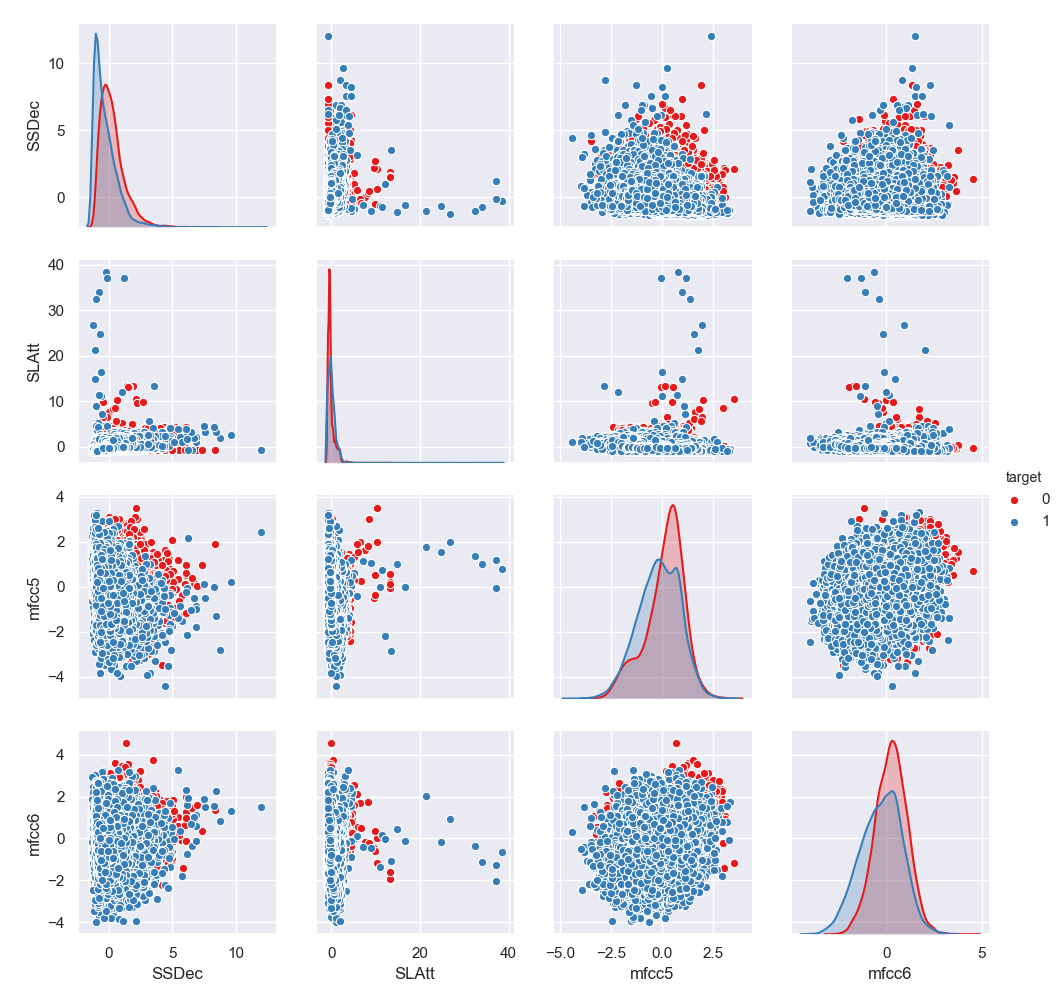
\includegraphics[width=0.7\textwidth]{res/figure_1.png}
\caption{Διαγράμματα συνδυασμών τεσσάρων χαρακτηριστικών ανά δύο}
\label{featureTable:table1}
\end{figure}


\section{Προεπεξεργασία δεδομένων}

Κατά την προεπεξεργασία των δεδομένων, δοκιμάστηκαν διάφορες τεχνικές έτσι ώστε να βρεθούν η βέλτιστη επιλογή χαρακτηριστικών και συνδυασμός μεθόδων. Οι μέθοδοι που δοκιμάστηκαν είναι η κλιμακοποίηση, κανονικοποίηση και ο συνδυασμός τους. Επίσης για την επιλογή των χαρακτηριστικών δοκιμάστηκαν το κατώφλι με βάση τη διακύμανση (VarianceThreshold) και η εκατοστιαία επιλογή (PercentileSelection), ενώ έγινε δοκιμή διάφορων τιμών των παραμέτρων αυτών των αλγορίθμων.

Τα αποτελέσματα παρουσιάζονται στον πίνακα \ref{table:tab}. Στην κλιμακοποίηση όλα τα χαρακτηριστικά έχουν μηδενικό μέσο και απόκλιση ίση με τη μονάδα ενώ στην κανονικοποίηση μετατοπίζονται οι τιμές τους ώστε να ανήκουν στο εύρος $[0,1]$. Τα VarianceThreshold και PercentileSelection, που είναι συναρτήσεις του sub-module feature\_selection της scikit-learn, αποκλείουν χαρακτηριστικά μέσω μετρικών αξιολόγησής τους. Στο VarianceThreshold, η μείωση του αριθμού των χαρακτηριστικών γίνεται με όρους διακύμανσης, δηλαδή αφαιρούνται όλα τα χαρακτηριστικά των οποίων η διακύμανση δεν ξεπερνά κάποιο κατώφλι, ενώ η PercentileSelection κατατάσσει τα χαρακτηριστικά με βάση τη διακριτική του ικανότητα και καταργεί όλα τα χαρακτηριστικά τα οποία βρίσκονται κάτω από ένα ποσοστό των καλύτερων καθορισμένο από το χρήστη.

\begin{table}[H]
	\centering
	\begin{tabular}{@{} l l r @{}}
		\toprule
		\textbf{Μοντέλο} & \textbf{Μέθοδοι προεπεξεργασίας} & \textbf{Ακρίβεια} \\ \midrule
		 & Χωρίς προεπεξεργασία & 0.49 \\
		 & Scaling & 0.89 \\
		 & Κανονικοποίηση & 0.49 \\
		 & Scaling και κανονικοποίηση & 0.78 \\
		 & VarThreshold και scaling & 0.88 \\
		 & PercenSel και scaling & 0.81 \\
		 & VarThreshold, scaling και gamma=scale & 0.88 \\
		 & VarThreshold, scaling και sigmoid kernel & 0.58 \\
		\multirow{-9}{*}{SVM} & VarThreshold,  scaling και polynomial kernel (5\textsuperscript{ου} βαθμού) & 0.84 \\ \midrule
		Decision Tree & VarThreshold και scaling & 0.75 \\ \midrule
		Multi-Layer Perceptron & VarThreshold, scaling και rndState = 2 & 0.86 \\ \midrule
		Naive Bayes & VarThreshold και scaling & 0.65 \\ \bottomrule
	\end{tabular}
	\caption{Μέθοδοι προεπεξεργασίας για διάφορα μοντέλα. \small
	Εδώ για συντομία όπου VarThreshold εννοείται VarianceThreshold, PercenSel εννοείται PercentileSelection και scaling εννοείται κλιμακοποίηση.}
	\label{table:tab}
\end{table}

Εν τέλει, αποφασίστηκε να χρησιμοποιηθεί μόνο η κλιμακοποίηση, επειδή η κανονικοποίηση δεν είχε κανένα αποτέλεσμα και το κέρδος σε ταχύτητα ταξινόμησης των παραπάνω τρόπων μείωσης του αριθμού χαρακτηριστικών δεν ήταν αρκετό συγκριτικά με την μείωση της ακρίβειας ώστε να δικαιολογήσει τη χρήση τους στην υλοποίηση. Βοήθησαν παρ' όλα αυτά στον προσδιορισμό των χαρακτηριστικών που υπερτερούν.

Στη συνέχεια, σε μία προσπάθεια περαιτέρω κατανόησης και κατάταξης των χαρακτηριστικών με βάση τη διακριτική τους ικανότητα, απομονώθηκαν όλα και ελέγχθηκε η ακρίβειά τους ένα ένα. Τα αποτελέσματα έδειξαν ότι, τελικά, κανένα χαρακτηριστικό από μόνο του δεν είναι ικανό να δώσει ικανοποιητικό ποσοστό ακρίβειας. Ακόμα και αν πάρουμε το καλύτερο σε όρους ακρίβειας και το δοκιμάσουμε σε συνδυασμό με τα επόμενα καλύτερα, φαίνεται ότι η ακρίβεια αυξάνεται λίγο αλλά όχι αρκετά. Τέλος, αν επαναληφθεί ακόμα μία φορά η διαδικασία, φαίνεται ότι έχουμε και πάλι μια μικρή αύξηση στην ακρίβεια, η οποία όμως είναι αρκετά μακρυά από την ακρίβεια που επιτυγχάνεται χρησιμοποιώντας όλα τα χαρακτηριστικά.

\begin{table}[H]
	\centering
	\begin{tabular}{@{} l r r r @{}}
		\toprule
		\textbf{Accuracy} & \textbf{Individually} & \textbf{With best first\textsuperscript{1}} & \textbf{With best second\textsuperscript{1}} \\ \midrule
		4Hz Mod & 0.58 & 0.66 & 0.73 \\
		Flat & 0.63 & 0.71 & 0.75 \\
		HFC & 0.58 & 0.65 & 0.72 \\ \midrule
		LAtt & 0.62 & 0.71 & 0.75 \\
		SC & 0.59 & 0.66 & 0.73 \\
		Scomp & 0.57 & 0.66 & 0.73 \\ \midrule
		SDec & 0.63 & 0.65 & 0.72 \\
		SEFlat & 0.51 & 0.65 & 0.72 \\
		SF & 0.55 & 0.69 & 0.75 \\ \midrule
		SFlat & 0.57 & 0.66 & 0.72 \\
		SLAtt & 0.63 & 0.71 & 0.74 \\
		SR & 0.60 & 0.66 & 0.72 \\ \midrule
		SSDec & \textbf{0.65} & - & - \\
		ZCR & 0.58 & 0.65 & 0.72 \\
		mfcc0 & 0.61 & 0.66 & 0.73 \\ \midrule
		mfcc1 & 0.58 & 0.67 & 0.73 \\
		mfcc2 & 0.52 & 0.66 & 0.73 \\
		mfcc3 & 0.56 & 0.69 & 0.76 \\ \midrule
		mfcc4 & 0.54 & 0.67 & 0.74 \\
		mfcc5 & 0.57 & 0.70 & 0.75 \\
		mfcc6 & 0.61 & \textbf{0.72} & - \\ \midrule
		mfcc7 & 0.57 & 0.68 & 0.75 \\
		mfcc8 & 0.55 & 0.67 & 0.74 \\
		mfcc9 & 0.54 & 0.67 & 0.73 \\ \midrule
		mfcc10 & 0.54 & 0.65 & 0.73 \\
		mfcc11 & 0.51 & 0.66 & 0.73 \\
		mfcc12 & 0.54 & 0.67 & 0.73 \\ \bottomrule
	\end{tabular}
	\caption{Ακρίβεια μεμονωμένων χαρακτηριστικών και συνδυασμών τους. \vspace{1em}\\\tiny
	1: όπου ``With best first'' εννοείται ο συνδυασμός του χαρακτηριστικού με το καλύτερο, ενώ ``With best second'' εννοείται ο συνδυασμός του χαρακτηριστικού με τον καλύτερο συνδυασμό που προέκυψε στο προηγούμενο βήμα}
\end{table}

Άρα, γίνεται προφανές ότι δεν υπάρχει κάποιο συγκεκριμένο, μοναδικό χαρακτηριστικό το οποίο ευθύνεται για το μεγαλύτερο ποσοστό της ακρίβειας του μοντέλου αλλά είναι ο συνδυασμός τους.
